   \footnote{This section is under development and should be considered unpublished.}

\section{History}

% caesar, one-time pad, substitution + transpostions + products thereof, etc.
\subsubsection{Substitution Ciphers}

One of the oldest known encryption algorithms is the so called Caesar cipher. It is said that he used it for communication with his army. It is a very simple character-wise substitution cipher. The idea is to substitute letters for each others.

\begin{example}[Caesar Cipher]
 In a very simple case the alphabet can be shifted by $3$ letters forward cyclically.
 Thus, \texttt{a} would be encrypted as \texttt{d}, \texttt{b} as \texttt{e}, \texttt{z} as \texttt{c}, etc.

 Below the lower row contains the encryption of the upper row. 
  \begin{lstlisting}
    meet me after the toga party
    phhw ph diwhu wkh wrjd sduwb
  \end{lstlisting}
\end{example}

Let us make this algorithm mathematically a bit more precise.
We usually represent all data as a number in $\Z_n$ so that encryption and decryption are functions $\Z_n\to\Z_n$.
$\Z_n$ is called the \textbf{alphabet}.
For the Latin alphabet, we have $n=26$, i.e., the letters are represented as the numbers $0, 1, 2,\ldots, 25$.

The length of the shift can be any number from $0$ to $25$.
It is very typical that an encryption scheme has such an arbitrary parameter.
Every choice of the parameter yields a different encryption function, and it is necessary to know that number to decrypt.
This number is called the \textbf{key}.

Now for a given key $k$, we can encrypt each letter $x$ as $\phi_k(x)=(x+k)\modop n$.
This is obviously, a very weak cipher.
Here, an attacker can easily try out all $26$ possible keys $k$ until the decryption of the message becomes a legible message.
Trying every possible key like this is called a \textbf{brute-force-attack}. 

We can generalize this approach of substituting the letters individually by different letters in the alphabet.
As the encryption function, we use an arbitrary bijection $\phi:\Sigma\to\Sigma$.
This is called a \textbf{substitution cipher}.
A \textbf{plaintext} or \textbf{message} is an element of $\Z_n^*$, i.e., a list of elements of the alphabet.
A plaintext is \textbf{encrypted} by applying $\phi$ to each element, which yields the \textbf{ciphertext}.

More precisely, this is called a \textbf{monoalphabetic} cipher.
There are $|\Sigma|!$ different bijections of a finite alphabet $\Sigma$, e.g., $26!\approx 4\times 10^{26}$ for the Latin alphabet.
So a brute force attack now seems very hard, and this looks like a strong cipher at first sight. 
However, monoalphabetic substitution ciphers can be attacked very efficiently because they do not obfuscate patterns in the plaintext---they encrypt the same plaintext with the same ciphertext every time.
In particular the same letter is always encrypted with the same letter. 
Thus, if the language of the message is known, the frequencies of occurrences of letters in the ciphertext can be correlated to the expected frequencies of occurrences of letters in the plaintext.
Then, if the ciphertext is long enough, only a few substitution remain likely and can be tried easily.

This is why \textbf{polyalphabetic} ciphers were introduced.
These map the same character differently depending on the position in the message where it occurs.

A simple polyalphabetic cipher is the Vigin\`ere cipher, a generalization of Caesar's cipher.
It splits the plaintext into blocks of $l$ characters.
So a text of length $l\cdot n$ would be split into $n$ blocks.
Then all letters are encrypted using Ceasar's cipher but using a different key depending on where in the block a character occurs.
Thus, the key is an $l$-tuple $k=(k_0,\ldots,k_{l-1})$.
For example, using $l=3$ and the key $(1,2,3)$, the block "aaa" becomes "bcd". 

\begin{example}[Vigin\`ere Cipher]
 We use blocks of length $l=3$ and the key $k=(1,2,3)$.
 Then we obtain the encryption
  \begin{lstlisting}
    meet me after the toga party
    nghu oh bhwft wig wpid qcuua
  \end{lstlisting}
\end{example}

\begin{exercise}\label{exc:sd:viginere}
Define the substitution function $\phi_k(i,x)$ of the Vigin\`ere cipher.
Given a key $k=(k_0,\ldots,k_{l-1})$, $\phi_k(i,x)$ should be the character that substitutes the character $x$ in position $i$.
\end{exercise}

This can be attacked by first looking for repetitive patterns in the ciphertext (in order to guess the length $l$ of the key) and attacking the decomposed Caesar-encrypted subsequences individually.
This works well if the length of the message is significantly longer than the length of the key. 

One notable special case arises when the length of the key equals the length of the message.
In this case we call the cipher a \textbf{one-time-pad}.
Then the encryption is absolutely secure as every ciphertext can be decrypted to an arbitrary plaintext by choosing an appropriate key.
The security of course only holds if the key is only used once---otherwise, it is effectively used to encrypt one very long message.
Therefore, one-time-pads have only limited use in practice: to send a second message, we have to transfer the new key secretly, which is as difficult as the original problem.
The only practical way to use a one-time-pad is to pre-agree on an extremely long key that is used up gradually as messages are sent.

\subsubsection{Permutation Ciphers}

A different approach is to \emph{rearrange} the letters of the message instead of substituting them.
That is called a \textbf{transposition} or \textbf{permutation} cipher.
An old example is the rail-fence permutation cipher.
Here a message is spelled out diagonally up and down over a number of rows, and the ciphertext is read off row-by-row.
The key $k$ is the number of rows.

\begin{example}[Rail-Fence Cipher]
 We use $k=3$.
 Then we obtain the following ciphertext:
  \begin{lstlisting}
    meet me after the toga party
    m aregaetm fe h oapryeettt t
  \end{lstlisting}
which is computed using the following visual aid where spaces are indicated as underscores.
  \begin{lstlisting}
   m   _   a   r   e   g   a

    e t m _ f e _ h _ o a p r y

     e   e   t   t   t   _   t
  \end{lstlisting}
\end{example}

A similar, more general class of ciphers are the route ciphers.
The plaintext is written out column-wise and then read back in a specific pattern (the route).
Each route defines a route cipher, and the number of rows $k$ is the key.

\begin{example}[Route Cipher]
Using $k=4$, writing out the plaintext column-wise yields
  \begin{lstlisting}
    m   a r e g a
    e m f     a r
    e e t t t   t
    t   e h o p y
  \end{lstlisting}

If we use the route ``top row, then alternating between second row and fourth row, then third row'', we obtain the same cipher as the rail-fence cipher for $k=3$.
\end{example}

Formally, a transposition cipher maps a plaintext $[x_0,\ldots,x_{m-1}]$ to $[x_{\tau(0)},\ldots,x_{\tau(l-1)}]$ where $\tau$ is a bijection of the positions $\{0,\ldots,l-1\}$ in the message.
To make the cipher parametric in a key, we use a function $\tau_k$ that maps keys $k$ to bijections.

\begin{exercise}\label{exc:sd:route}
Consider the route cipher for the route ``row-wise starting with top row''.
Define the resulting bijection $\tau_k$ of $\{0,\ldots,l-1\}$ mathematically.
Also give the inverse of $\tau_k$ (which is needed for decryption).
\end{exercise}

Transposition ciphers do not really obfuscate plaintext patterns either.
For instance, the number of occurrences of the letters remain unchanged by the cipher.

\subsubsection{Product Ciphers}
 
A good way to produce more secure encryptions is to compose multiple ciphers.
The resulting ciphers are called \textbf{product} ciphers.
If we compose a substitution cipher with another substitution cipher, we obtain a substitution cipher again, which is nothing new.
Similarly, if we compose two permutation ciphers, we get a permutation cipher again.

However, if we compose a substitution and a permutation, we get a new kind of cipher that is much harder to break.
This is a key idea in modern (symmetric) cryptography. 


\section{Preliminaries}

\begin{definition}[polynomial-time algorithm]
 An algorithm $A$ is called polynomial time algorithm iff there exists $k\in \mathbb{N}$ such that the maximum number $t$ of operations $A$ has to perform for input of length $n$ satisfies $t(n)\in O(n^k)$.
\end{definition}

\begin{definition}[A probabilistic polynomial-time algorithm]
 A probabilistic polynomial-time algorithm (PPT) is a polynomial-time algorithm that might be non-deterministic. If it is deterministic we will just call it polynomial time algorithm.
\end{definition}

\begin{definition}
 A function $f:\,\mathbb{N}\to\mathbb{R}$ is called negligible iff $$\forall k\in\mathbb{N}.\,\exists N_k\in\mathbb{N}.\,\forall n\geq N_k:\,n\left|f(n)\right|<1.$$
\end{definition}

One important cryptographic primitive is the so called one-way function (OWF). Using these one-way-functions one can build provably secure symmetric encryption algorithms. However, it is currently not known whether there exist any one-way function. In the following we will especially consider one-way permutations (OWP), bijective OWFs with identical input and output length. 

\begin{definition}[One way function]
 A function $f:\{0,1\}^*\to \{0,1\}^*$, is called a one-way function iff, $f$ is a PPT and for any natural number $n$ and any PPT $A$, there is a negligible function $neg$ such that: $$\mathrm{Pr}\left[f(A(f(x),1^n))=f(x)\right]\leq neg,$$ where $x$ is chosen uniformly random.
\end{definition}
Intuitively, OWFs are simply hard to invert PPTs. Some functions that are commonly believed to be OWFs are modular exponentiation and the multiplication of big prime numbers. 
%\vdots\ \\
%One way permutations\\\vdots\ \\

Another important concept is the so called Pseudo-random generator (PRG or PRNG). 
\begin{definition}[PRGs]
 A function $H:\{0,1\}^*\to \{0,1\}^*$ is called PRG iff:
 \begin{itemize}
  \item $H$ is a PPT
  \item There exists a PPT the so called \emph{length extension function} $l:\mathbb{N}\to\mathbb{N}$, s.t. $\forall n\in\mathbb{N}.\,l(n)>n\land \left|H(x)\right|=l(\left|x\right|), \forall x\in\{0,1\}^*$
  \item There is a negligible function $neg$ s.t. for any PPT $A$, we have:
  $$\left|\mathrm{Pr}\left[A(H(U_n))=1\right]-\mathrm{Pr}\left[D(U_{l(n)})=1\right]\right|<neg(n),$$ where $U_k$ denotes a uniformly random element of $\{0,1\}^k$. 
 \end{itemize}
\end{definition}

It can be shown that given any OWF, we can build a PRG. %TODO: Insert a proof for at least OWPs using hard core bits
%This part should probably be moved to the appendix
\begin{definition}[hard-core bit]
 Let $f$ be a one-way function. Now the function $b:\{0,1\}^*\to\{0,1\}$ is called a \emph{hard-core bit} for $f$ if $b$ is computable in polynomial time and there exists a negligible function $neg(n)$ such that for any $n\in\\mathbb{N}$ and any PPT $A$:
 $$\mathrm{Pr}\left[A(f(x),1)=b(x)\right]\leq\frac{1}{2}+neg(n), $$ where $x\in\{0,1\}$ uniformly random. 
\end{definition}

The next step is to find one-way functions (assuming that there are one-way functions at all) for which we can build hard-core bits. 
\begin{theorem}
 Let $f$ be a one-way function. Define $g:\{0,1\}^{2n}\to\{0,1\}^*$ as $g(x\circ y)=f(x)\circ y$, where $\left|x\right|=\left|y\right|=n$. Then $g$ is a one-way function with hard-core bit $$b(x,y)=\bigoplus_{i=1}^n x_i\land y_i=\sum_{i=1}^{n}x_iy_i (\mod 2).$$
\end{theorem}
If now $f$ was a one-way permutation, we can use the above construction to get an additional pseudo-random bit, so we already have a pseudo-random generator.


\section{Hashing}

\subsection{MDx}

\subsection{SHA-x}


\section{Symmetric Encryption}
The basic principle of symmetric encryption is that encryption and decryption use the same key.

\subsection{Schemes}

We now expand on the ideas developed in Sect.~\ref{sec:sd:crypto:hist} systematically.

\begin{definition}[Encryption Scheme]
 An \textbf{encryption scheme} is a tuple $(\Sigma,K,G, E, D)$, where
  \begin{compactitem}
   \item $\Sigma$ is a (finite) set (the \textbf{alphabet}),
   \item $K=(K_n)_{n\in \N}$ is a family of sets (the \textbf{key space}),
   \item $G:(n\in \N)\to K_n$ is a PPT algorithm (the \textbf{key generation} function)
   \item $E=(E_k)_{n\in\N,k\in K_n}$ is a family of polynomial algorithms $E_k:\Sigma^n\to\Sigma^*$ (the \textbf{encryption} functions)
   \item $D=(D_k)_{n\in\N,k\in K_n}$ is a family of (possibly partial) polynomial algorithms $D_k:\Sigma^*\to\Sigma^n$ (the \textbf{decryption} functions)
  \end{compactitem}
  such that for all $n\in N$, $k\in K_n$, and $x\in \Sigma^n$, we have $D_k(E_k(x))=x$.

  For $x\in\Sigma^n$, we write $E(x)$ for the probabilistic result of computing $E_{G(n)}(x)$.
\end{definition}

To encrypt a message $x$ of length $n$, we choose a key $k=G(n)\in K_n$ and call $c=E_k(x)$ to obtain the cipher $c$.
To decrypt an encrypted message, we call $D_k(c)$.

\subsection{Security of a Scheme}

There are various concepts of security of an encryption scheme.
The general idea is to assume an adversary that picks two messages $x_0,x_1\in\Sigma^n$ and randomly receives either $E(x)$ or $E(x')$.
The encryption scheme is considered secure if the adversary cannot distinguish between the two situations with a probability that is non-negligibly better than $1/2$.
In other words, even if the adversary already knows that a given ciphertext $c$ is either the encryption of $x$ or of $x'$, he has no better chance of decrypting $c$ than guessing.

In all cases, the adversary is restricted to polynomial computations.
But we obtain different notions of security depending on how we model what else the adversary is allowed to do.

In the simplest case, the adversary may do nothing else:

\begin{definition}[Computationally-indistinguishable]\label{def:sd:ind}
  An encryption scheme $(\Sigma,K,G,E,D)$ is \textbf{computationally-indistinguishable} (comp-ind) if for any PPT $A:\Sigma^*\to\{0,1\}$, messages $x_0,x_1\in\Sigma^n$, and $n\in \N$
  \[\Prob{i\in\{0,1\}}{A(E(x_i))=i}<\frac{1}{2}+neg(n)\]
  for a negligible function $neg$.
\end{definition}

Here $\Prob{i\in\{0,1\}}{A(E(x_i))=i}$ formalizes the probability that the adversary correctly guessed whether $x_0$ or $x_1$ is the decryption of its input.

\begin{example}
A monoalphabetic substitution cipher is not secure in the sense of Def.~\ref{def:sd:ind}.
We define an adversary $A$.
Given the encryption $c$ of $x_0$ or $x_1$, $A$ collects the frequencies of all characters in $c$.
If those frequencies match the frequencies in $x_0$ or $x_1$, $A$ guesses $0$ or $1$, respectively.
Clearly, $A$ is a polynomial algorithm.
\end{example}

comp-ind is still a relatively weak notion of security because a realistic adversary may have access to the encryption scheme and may try to reverse-engineer it in some way.
If the adversary has access to the encryption function $E(-)$, we speak of a \textbf{chosen-plaintext-attack} (CPA).
The analog of Def.~\ref{def:sd:ind} where the adversary $A$ may conduct CPAs is called CPA-ind.
If the adversary additionally has access to the decryption function $D(-)$, we speak of \textbf{chosen-ciphertext-attack} (CCA).
The analog of Def.~\ref{def:sd:ind} where the adversary $A$ may conduct CCAs as well is called CCA-ind.

\begin{example}
Let $\Sigma=\{0,1\}$.
We consider every natural number to be an element of $\{0,1\}^*$ by using its binary representation.

Given a PRG $R$, we can iterate it on its own output to get an arbitrarily long pseudo-random element of $\{0,1\}^*$.
Now we can construct an encryption scheme by simply defining
\begin{compactitem}
 \item the key generator by $G(n)=R(n)$
 \item $E_k(x)$ by xor-ing every bit in $x$ with the corresponding bit in $k$.
 \item the decryption in the same way as encryption, i.e., $D_k=E_k$.
\end{compactitem}

The resulting encryption scheme is comp-ind but not necessarily CPA-ind.
\end{example}

\subsection{Schemes Based on Block Ciphers}

We fix the alphabet to be $B=\{0,1\}$.

Symmetric encryption is a wide field with a rich set of mathematical background and very sophisticated algorithms.
Therefore, we can only cover a small fragment of the topic.
Concretely, we describe:
\begin{compactitem}
 \item the general principle of building encryption schemes from block ciphers
 (see also \url{https://en.wikipedia.org/wiki/Block_cipher})
 \item substitution-permutation networks as an example of a general class of relatively simple block ciphers
 (see also \url{https://en.wikipedia.org/wiki/Substitution-permutation_network})
 \item the AES block cipher as an example of a sophisticated practical substitution-permutation network
 (see also \url{https://en.wikipedia.org/wiki/Advanced_Encryption_Standard})
\end{compactitem}

\subsubsection{Block Ciphers and Modes of Operation}

Block ciphers are a common method to obtain more secure encryption schemes.
They pick up on the ideas from Sect.~\ref{sec:sd:crypto:hist}, specifically the use of product ciphers that combine substitutions and permutations, and develop them further.

\paragraph{Block Ciphers}
A \textbf{block cipher} is a function that maps keys to bijections of the set $B^N$ for some $N$.
The elements of $B^N$ are called \textbf{blocks}.

The idea of block cipher--based schemes is to split the plaintext into blocks that are encrypted individually by applying the block cipher.
The last block may have to be \textbf{padded} to length $N$ by adding, e.g., zeros or random data.

\paragraph{Mode of Operation}
However, the naive approach would not yield secure schemes---if the same block is always encrypted in the same way, the scheme would be easy to attack.
Overcoming this is the role of the block cipher \textbf{mode of operation}.
There are various modes that yield CPA-ind secure schemes if used with pseudo-random block ciphers.

\paragraph{Cipher Block Chaining}
A commonly used mode of operation is \textbf{Cipher Block Chaining} (CBC).
Here every plaintext block is xor-ed with an element from $B^N$ before applying the block cipher.
For the first plaintext block, this is an arbitrary number called the \textbf{initialization vector} (IV).
For every subsequent plaintext block, it is the previous cipher block.

Fig.~\ref{fig:sd:cbc} shows the data flow for $N=8$ and $3$ successive plaintext blocks (where $\oplus$ indicates bit-wise xor).

\paragraph{Initialization Vector}
The IV does not have to be secret (which is good because the recipient needs to know it to decrypt).
For some modes of operation that use IVs, the IV can simply be a counter, e.g., the number of the current message in the overall sequence of exchanged messages.

However, for CBC, it is important that the IV is unpredictable to the adversary.
So it is usually chosen randomly, which makes CBC encryption a probabilistic algorithm.
Moreover, to maintain security, the same pair of initialization vector and key must never be used twice, i.e., the initialization vector should be a number only used once (which is called a \textbf{nonce}).

Choosing the IV randomly raises the question how the recipient learns about the IV in order to decrypt.
There are several options:
\begin{compactitem}
 \item The sender sends the IV (unencrypted) along with the first message. The IV can be public as long as it is random.
 \item Sender and recipient use the exact same PRG so that they can compute the IV separately.
 \item The recipient ignores the first ciphertext block. As seen in Fig.~\ref{fig:sd:cbc}, in CBC mode, the recipient only needs the IV to decrypt the first block.
\end{compactitem}

\begin{figure}[htb]
\begin{center}
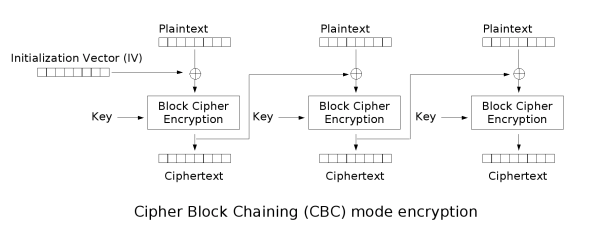
\includegraphics[width=.5\textwidth]{Cbc_encryption.png}
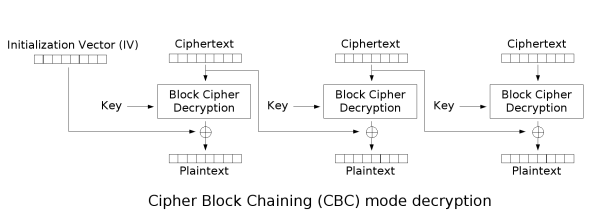
\includegraphics[width=.5\textwidth]{Cbc_decryption.png}
\end{center}
\caption{Data Flow in CBC Mode\protect\footnotemark}\label{fig:sd:cbc}
\end{figure}
\footnotetext{Images By WhiteTimberwolf (SVG version)---PNG version, Public Domain, \url{https://commons.wikimedia.org/w/index.php?curid=26434095} and \url{https://commons.wikimedia.org/w/index.php?curid=26434096}}


%\subsubsection{Feistel Ciphers}
%
%For this we can use a so called Feistel network.
%%Improving a comp. ind. encryption scheme to an ind. CPA secure scheme using a Feistel-network.
%\begin{definition}[A Feistel cipher]
% Let $k$ be any natural number (the number of \emph{rounds}). Let $f_{k_i}$ be a family of functions\protect\footnote{If possible pseudorandom functions and possibly one-way functions.} ($f$ is the so called \emph{round function}) of output length $n$ indexed by the sequence of \emph{round keys} $k_1, k_2, \ldots, k_n$. 
% Then the following encryption algorithm $E_k$ is called Feistel cipher. %network with $k$ iterations (for some odd $k$) based on a pseudo random generator $f_{k_i}$ and round keys $k_1, k_2, \ldots, k_n$ is an encryption scheme $(G,E,D)$, defined by:
% %For any odd $k\in\mathbb{N}$ we call an encryption scheme $(G, E, D)$ a Feistel network with $k$ iterations and $P$-Box $f$, iff for some \emph{round keys} $k_1, k_2, \ldots, k_n$ used as input for the pseudo random generator $f_{k_i}$. 
% \begin{itemize}
%  \item Fix a message $m=:x_1\circ x_2$, where $\left|x_1\right|=\left|x_2\right|=n$
%  \item Define the sequences $L_1, L_2, \ldots, L_n$ and $R_1, R_2, \ldots, R_n$ by $L_1:=x_1, R_1:=x_2$ and $L_{n+1}:=R_n, R_{n+1}:=L_n\oplus f_{k_n}(R_n)$. Finally define $E_k:x_1\circ x_2\to L_k\circ R_k$. 
% \end{itemize}
% Now we can define the corresponding decryption algorithm $D_k$ just like $e_k$, but with the reversed order of round keys:
% \begin{itemize}
%   \item Fix a ciphertext $c=:x_1\circ x_2$, where $\left|x_1\right|=\left|x_2\right|=n$
%   \item Define the sequences $L_1, L_2, \ldots, L_n$ and $R_1, R_2, \ldots, R_n$ by $L_1:=x_1, R_1:=x_2$ and $L_{n+1}:=R_n, R_{n+1}:=L_n\oplus f_{k_{k-n}}(R_n)$. Finally define $D_k:x_1\circ x_2\to L_k\circ R_k$. 
% \end{itemize}
%\end{definition}
%Feistel ciphers have been shown to fulfill several notions of security assuming that the round function is actually pseudo random. For instance Feistel networks with at least $3$ rounds are ind. CPA secure and for more rounds they fulfill even stronger notions of security. %  TODO: Check and clearify the exact model (3 seems sufficient under some assumptions, but 4 is definitely better (and already fulfills stronger notions)) and perhaps mention some other results. %see \url{https://link.springer.com/chapter/10.1007/978-3-540-45146-4\_30}

\subsubsection{Substitution-Permutation Networks}

A substitution-permutation network is a block cipher whose bijections arise as products of substitution and permutation ciphers.

To process a block of $N$ bits, the block is divided into $b$ chunks of $n=N/b$ bits each.
Each block is processed by a sequence of steps, each of which applies a bijection $B^N\to B^N$.

There are different kinds of steps:
\begin{itemize}
\item A \textbf{substitution step} consists of $b$ bijections $B^n\to B^n$, called \textbf{S-boxes}.
The substitution step maps each chunk by applying the corresponding S-box.

This expands on the ideas of polyalphabetic substitution ciphers from Sect.~\ref{sec:sd:crypto:hist}.
It substitutes each $n$-bit chunk by another chunk, and each chunk is substituted using a different substitution.

It is desirable to have every output bit of an S-box depend on \emph{every} input bit.
Then changing one input bit maximally \textbf{confuses} the output.

\item A \textbf{permutation step} consists of a permutation of $\{0,\ldots,N-1\}$, called a \textbf{P-box}.

The permutation step maps the entire block at once by permuting its bits according to the P-box.
This corresponds to a transposition cipher from Sect.~\ref{sec:sd:crypto:hist}.

It is desirable that the bits of one chunk are rearranged to as many different chunks as possible.
That maximizes the \textbf{diffusion} of bits among the chunks.

\item A \textbf{key step} consists of a number $k\in B^N$, called a \textbf{key}.
The key step maps a block by xor-ing it with $k$.

The key steps provide a way to parametrize the network.
We can use the same network multiple times by just switching to a different set of keys.
\end{itemize}

A \textbf{round} is a bijection of $B^N$ that is the product of some substitution and permutation steps and usually one key step.

A \textbf{network} is a sequence of rounds.
Often the substitution and permutation steps are the same for each round, and only the key of the key step changes between rounds.
In the simplest non-trivial case, the network consists of $b$ S-boxes (making up one substitution step), followed by one P-box, followed by one key step.
The more keys are available, the more rounds can be run, the more secure the network.

The inverse of a network is defined by inverting all operations in reverse order.

\begin{example}[Substitution-Permutation Network]\label{ex:sd:spn}
Fig.~\ref{fig:sd:subpernet} shows a Substitution-Permutation Network.
It uses $N=16$ and $b=n=4$.
Its rounds consists of one substitution step (using $4$ S-boxes), one permutation step (using P-box $P$), and one key step.

$4$ rounds are concatenated using keys $K_0,\ldots,K_3$ that are obtained from one overall key.
The first round only uses the key step, and the last round skips the permutation step.
\end{example}

\begin{figure}[htb]
\begin{center}
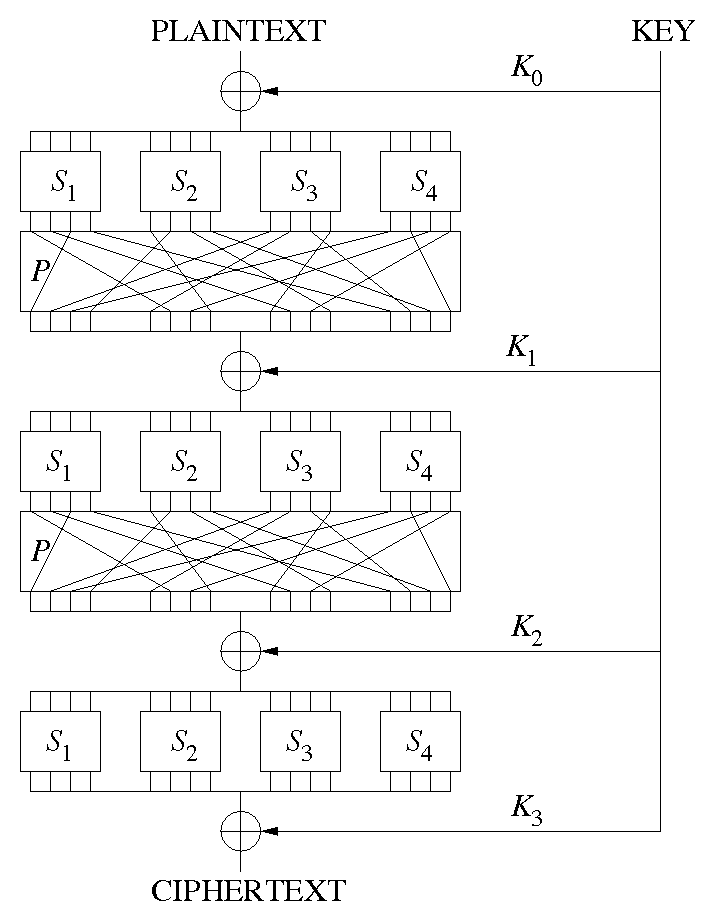
\includegraphics[width=.5\textwidth]{SubstitutionPermutationNetwork.png}
\end{center}
\caption{A simple Substitution-Permutation-Network\protect\footnotemark}\label{fig:sd:subpernet}
\end{figure}
\footnotetext{Image by GaborPete---Own work, CC BY-SA 3.0, \url{https://commons.wikimedia.org/w/index.php?curid=6420152}}

\begin{exercise}\label{exc:sd:spn}
Consider the network for $N=8$ and $b=2$, whose rounds consist of the following steps:
\begin{compactenum}
 \item Substitution step consisting of the S-box $S=S_1=S_2$.
  The substitution $S:B^4\to B^4$ is given by $x\longmapsto ((x+1)\cdot 7)\modop 17-1$.
  This is a bijection of $B^4$, where $4$-bit chunks are seen as natural numbers via their binary encoding.
 \item Permutation step consisting of the P-box $P:B^8\to B^8$, which does a cyclic $2$-bit left-shift of its argument.
 \item Key step with $8$-bit key $k_i$ where $i$ is the number of the round.
\end{compactenum}
The network consists of two rounds using a $16$-bit key $k$, whose first $8$ bits are $k_1$ and whose last $8$ bits are $k_2$.

We obtain an encryption scheme by using CBC mode with an IV that is generated randomly.

Assume the key is $1001\,1000\,0010\,0110$.

Manually encrypt the plaintext \texttt{abc} (seen as $3$ blocks of $8$ bits using ASCII encoding), assuming the IV is $1010\,1010$.

Decrypt the ciphertext again.
\end{exercise}


%Substitution-permutation-network and Feistel networks using $S$-Boxes are quite similar.
%Ciphers based on substitution-permutation-networks can be better parallelized, but Feistel ciphers can use any pseudo-random function (for instance any one-way function) and are therefore limited to invertible ($P$-Boxes). %Also the Feistel networks can be adapted to ciphers not using blocks (for instance it is used in OAEP).

\subsubsection{AES}

\paragraph{Overview}
AES (Advanced Encryption Standard) was chosen by NIST (the US institute of standards and technology) in 2001 as an encryption standard after an open call in 1997 and extensive analysis of the submitted schemes.
Before being adopted as AES, it was called Rijndael.
It replaced DES, which was not secure anymore.

AES is one of the most widely used block ciphers, approved by many government organizations.
Implementations are available in many programming languages.

AES uses a substitution-permutation network for $N=128$, $b=16$, and $n=8$.

\paragraph{Keys}
While Rijndael is very flexible, NIST chose only three special cases for AES.
They differ mainly by the key size and the number of rounds:
\begin{center}
  \begin{tabular}{|c|c|c|c|}
  	\hline key size & 128-bit & 192-bit & 256-bit \\ 
  	\hline number of rounds & 10 & 12 & 14 \\ 
  	\hline
  \end{tabular}
\end{center}
In all three cases, one additional initial round is run that only xors the input with a round key.

Thus, $11$, $13$, or $15$ $128$-bit round keys $k_0,\ldots,k_r$ for $r\in\{10,12,14\}$ are needed.
These are obtained from the overall key using the Rijndael key schedule, which we omit here.

\paragraph{Details}
The substitution-permutation network of AES looks as follows:
\begin{compactenum}
 \item Round 0: key step with $k_0$
 \item Round $i$ for $i=1,\ldots,r-1$:
  \begin{compactenum}
    \item substitution step (called \emph{sub-bytes}) with a fixed $8$-bit S-box used $16$ times
    \item permutation step (called \emph{shift-row}) with a fixed permutation of $128$ bits
    \item substitution step (called \emph{mix-columns}) with a fixed $32$-bit S-box used $4$ times
    \item key step (called \emph{add-round-key}) with key $k_i$
  \end{compactenum}
 \item Round $r$: as before but without the mix-columns step
\end{compactenum}

The $128$-bit block to be mapped is represented as $16$ chunks of $8$ bits.
The chunks are arranged as a $4\times 4$ matrix.
The $4$ basic steps are defined as follows:
\begin{compactitem}
  \item sub-bytes: This substitution step applies a fixed S-box (the Rijndael S-box, which we omit here) to every chunk.
  \item shift-row: This permutation step leaves the chunks as they are but rearranges them relative to each other.
    Specifically, for $i=0,1,2,3$, the $i$-th row of the matrix is left-shifted cyclically $i$ times.
  \item mix-columns: This is a more complex step that applies the same fixed substitution to each column of the matrix.
    Thus, this step can be seen as a substitution step using $4$ chunks of size $32$, and using the same fixed S-box $4$ times.
    
    The fixed S-box is defined as follows.
    A column consists of $4$ bytes, each of which can be seen as an element of $F_{2^8}$ (see Sect.~\ref{sec:math:finfield} for finite fields).
    Thus, a column of $32$ bits can be seen as a $4$-dimensional vector over $F_{2^8}$.
    This vector is multiplied with the fixed $4\times 4$ matrix over $F_{2^8}$ given by
    \[\left(\begin{matrix}
    2&3&1&1\\1&2&3&1\\1&1&2&3\\3&1&1&2
   \end{matrix}\right)\]
  \item add-round-key: This key steps xors all $128$ with the respective round key.
\end{compactitem}

% substitution, one-time pad, DES

\section{Asymmetric Encryption}

The idea behind RSA is that if $N=p\cdot q$ for large prime numbers $p$ and $q$, it is very difficult to compute $p$ and $q$ from $n$.

\subsection{RSA}

\paragraph{Setup}
Choose two large primes $p$ and $q$ (typically of roughly equal size).
Put $N=p\cdot q$.

Now put $n=(p-1)(q-1)$. (Actually, any common multiple of the two numbers is fine.)
Note that $n=\phi(N)$.
Pick $e\in Z_n$ such that there is a $d\in\Z_n$ with $e\cdot d\Equiv_n 1$.
Such a $d$ exists if $\gcd(e,n)=1$ and is easy to compute (see Thm.~\ref{thm:math:extendedeuclid}).

The keys are defined as follows:
\begin{compactitem}
 \item public information (encryption key): $N$ and $e$
 \item private information (decryption key): $n$, $d$, $p$, and $q$
\end{compactitem}
Among the private information, only $N$ and $d$ are needed later on.
So $n$, $p$, and $q$ can be forgotten.
But they have to remain private---$p$ (or $q$) is enough to compute $n$ and $d$.

Different keys are often compared by their size.
That size is the number of bits in $N$.

\paragraph{Encryption}
Messages are numbers $x\in F_N$.
For example, we can choose the largest $k$ such that $2^k<N$ and use $k$-bit messages.

Encryption and decryption are functions $\Z_N\to \Z_N$ given by
\begin{compactitem}
 \item encryption: $x\mapsto x^e\modop N$
 \item decryption: $x\mapsto x^d\modop N$
\end{compactitem}

These are indeed inverse to each other:

\begin{theorem}
For all $x\in Z_N$, we have $(x^d)^e\Equiv_N (x^e)^d \Equiv_N x$.
\end{theorem}
\begin{proof}
In general, because $N=p\cdot q$ for prime numbers $p$ and $q$, we have that $x\Equiv_N y$ iff $x\Equiv_p y$ and $x\Equiv_q y$.

So we have to show that $x^{de}\Equiv_p x$.
(We also have to show the same result for $q$, but the proof is the same.)
We distinguish two cases:
\begin{compactitem}
\item $p|x$: Then trivially $x^{de}\Equiv_p x\Equiv_p 0$.
\item Otherwise. Then $p$ and $x$ are coprime.\\
   By construction of $e$ and $d$ and using Thm.~\ref{thm:math:extendedeuclid}, we have $k\in\N$ such that $e\cdot d+k\cdot n=1$.
   Thus, we have to show $x^{de}=x\cdot (x^{p-1})^{k\cdot(q-1)}\Equiv_p x$.
   That follows from $x^{p-1}\Equiv_p 1$ as known from Thm.~\ref{thm:math:fermatlittle}.
\end{compactitem}
\end{proof}

\paragraph{Attacks}
To break RSA, $d$ has to be computed.
There are $3$ natural ways to do that:
\begin{compactitem}
 \item Factor $N$ into $p$ and $q$. Then compute $d$ easily.
 \item Compute $n$ using $n=\phi(N)$ (which may be easier than finding $p$ and $q$). Then compute $d$ easily.
 \item Find $d$ such that $e\cdot d\Equiv_n 1$ (which may be easier than finding $n$).
\end{compactitem}
Currently these are believed to be equally hard.

It is believed that there is no algorithm for factoring $N$ that is polynomial in the number of bits of $N$.
That is no proved.
There are hypothetical machines (e.g., quantum computers) that can factor $N$ polynomially.

Note that checking if $N$ can be factored (without producing the factors) is polynomial, and practical algorithms exist (in particular, the AKS algorithms).
That is important to find the large prime number $p$ and $q$ efficiently.
\medskip

If there is indeed no polynomial algorithm, factoring relies on brute-force attacks that find all prime numbers $k<\sqrt{N}$ and test $k|N$.
Therefore, larger keys are harder than break to smaller ones.
Because of improving hardware, the key size that is considered secure grows over time.

Keys of size $1024$ are considered secure today, but because security is a relative term, keys of size $2048$ are often recommended. 
%It is quetionable that 1024-bit rsa is really secure, even though it has not yet been publicly broken;
%(see for instance https://en.wikipedia.org/wiki/RSA_%28cryptosystem%29#Integer_factorization_and_RSA_problem or https: //www.schneier.com/blog/archives/2007/05/307digit_number.html).
Larger keys are especially important if data is needed to remain secure far into the future, when faster hardware will be available.

\section{Authentication}

\section{Key Generation and Distribution}

   % security protocol correctness, such as key management protocol correctness,
   % e.g., going back to the work by Burrows, Abadi, and Needham on a logic of authentication (https://doi.org/10.1145/77648.77649)
   % Its an application of logic to a concrete problem space where errors are obviously bad.
